\documentclass{article}

\usepackage{amsmath}
\usepackage{listings}
\usepackage{amsfonts}
\usepackage{amssymb}
\usepackage{xcolor}
\usepackage{graphicx}
\usepackage{titling}
\usepackage[utf8]{inputenc}
\usepackage[english]{babel}
\usepackage{amsmath}
\usepackage{fancyhdr}
\usepackage{lastpage}
\usepackage{textcomp}
\usepackage{graphicx}
\usepackage{hyperref}
\usepackage{float}

\addtolength{\oddsidemargin}{-.875in}
\addtolength{\evensidemargin}{-.875in}
\addtolength{\textwidth}{1.75in}
\addtolength{\topmargin}{-.875in}
\addtolength{\textheight}{1.75in}

\title{\Huge Applicazioni delle reti telematiche \vspace{1cm}}
\author{Edoardo Terzi, Alessandro Bianchi, Davide Bertacco, Luca Giussani, Paolo Fiori, Davide Taurisano, \\
Giovanni Converso, Jonathan De Boni, Eric Palmas, Kevin Dominguez, Marco Maccarini.\vspace{0.5cm}}
\date{Semestre primaverile 2019}
\setcounter{page}{0}
\pagestyle{fancy}
\fancyhf{}

\fancyfoot[C]{Page \thepage \hspace{1pt} of \pageref{LastPage}}


\begin{document}

\maketitle
\thispagestyle{empty}
\pagebreak

\tableofcontents
\lstset{language=C++}
\pagebreak

\section{SDH ATM MPLS}

\section{Metasploit}
\subsection{Teoria}
\subsubsection{Penetration Test}
Il penetration test è il processo operativo di valutazione della sicurezza di un sistema o di una rete che 
simula l'attacco di un utente malintenzionato. L'analisi comprende più fasi ed ha come obiettivo evidenziare 
le debolezze della piattaforma fornendo il maggior numero di informazioni sulle vulnerabilità che ne hanno 
permesso l'accesso non autorizzato. L'analisi è condotta dal punto di vista di un potenziale attaccante e 
consiste nello sfruttamento delle vulnerabilità rilevate al fine di ottenere più informazioni possibili 
per accedere indebitamente al sistema. Il penetration test fornisce una stima chiara sulle capacità di 
difesa e del livello di penetrazione raggiunto nei confronti: 
\begin{itemize}
    \item delle vulnerabilità interne al sistema,
    \item delle vulnerabilità esterne al sistema,
    \item della sicurezza fisica.
\end{itemize}
\subsubsection{Procedura Black \& White Box}
I processi di penetration test possono essere effettuati in diverse modalità. La differenza consiste 
sulla quantità e qualità delle informazioni disponibili agli analisti riguardo ai sistemi analizzati.
\begin{itemize}
    \item \textbf{Black Box:} non presuppongono precedente conoscenza dell'infrastruttura oggetto di analisi 
    e gli esaminatori necessitano di determinare architettura e servizi dei sistemi prima di iniziare l'analisi.
    \item \textbf{White Box:} sono invece fornite conoscenze dettagliate dell'infrastruttura da esaminare, 
    spesso comprensive di schemi di rete, codice sorgente delle applicazioni e liste di indirizzi IP presenti nella rete.
    \item \textbf{Grey Box:} sono varianti a queste metodologie.
\end{itemize}
\subsubsection{Analisi dell’architettura e rilevazione delle vulnerabilità}
Vengono acquisite inizialmente le informazioni principali sull'architettura della piattaforma e sui servizi 
offerti. Dall'analisi di questi dati deriva la scelta di come condurre il passo successivo, consistente in 
una enumerazione dei principali errori e problemi. 
\subsubsection{Attacco e redazione di un report}
L'attività si conclude nello sviluppo della reportistica composta dal report di analisi sommaria dedicato 
al management o executive summary, contenente l'analisi dell'impatto di rischio di quanto riscontrato e 
tempistiche per l'azione di rientro o mitigazione delle problematiche riscontrate, e dal report tecnico, 
contenente l'analisi dettagliata dei problemi e la soluzione tecnica. 
\subsubsection{OS per il penetration test}
Kali, Parrot Security OS, BlackBox, BlackArch, Samurai Web Testing Framework 
\subsubsection{Kali linux}
OS basato sulla distribuzione Debian GNU/Linux, permette di testare penetration testing OS, rewrite of 
BackTrack Linux e sviluppare sicurezza preventiva o offensiva. Ha più di 300 tool di supporto, è 
multilingua, è personalizzabile e flessibile, e ha una grande community per il supporto. \\
\pagebreak
\paragraph{Tool principali:} 
\begin{itemize}
    \item Metasploit: security assesment framework
    \item NMAP: network scanner 
    \item John The Ripper \& Hashcat: password cracker
    \item Aircrack-ng: Wi-Fi crack
    \item Hydra: brute force attacks
    \item Maltego: information gathering
    \item Nikto: web scanner
    \item SET: Social Engineering Toolkit
    \item Bettercap: MITM attacks 
\end{itemize}
\subsubsection{Metasploit framework}
Si tratta di uno strumento open source per lo sviluppo e l'esecuzione di exploits ai danni di una macchina 
remota. È caratterizzato da: interfaccia a linea di comando, import da terze parti, exploitation manuale e 
azioni di forza bruta anch’esse condotte manualmente. Questa versione di Metasploit Project include anche 
Zenmap, un famoso port scanner, e un compilatore per Ruby, il linguaggio usato per questa versione. 
\begin{figure}[H]
    \center
    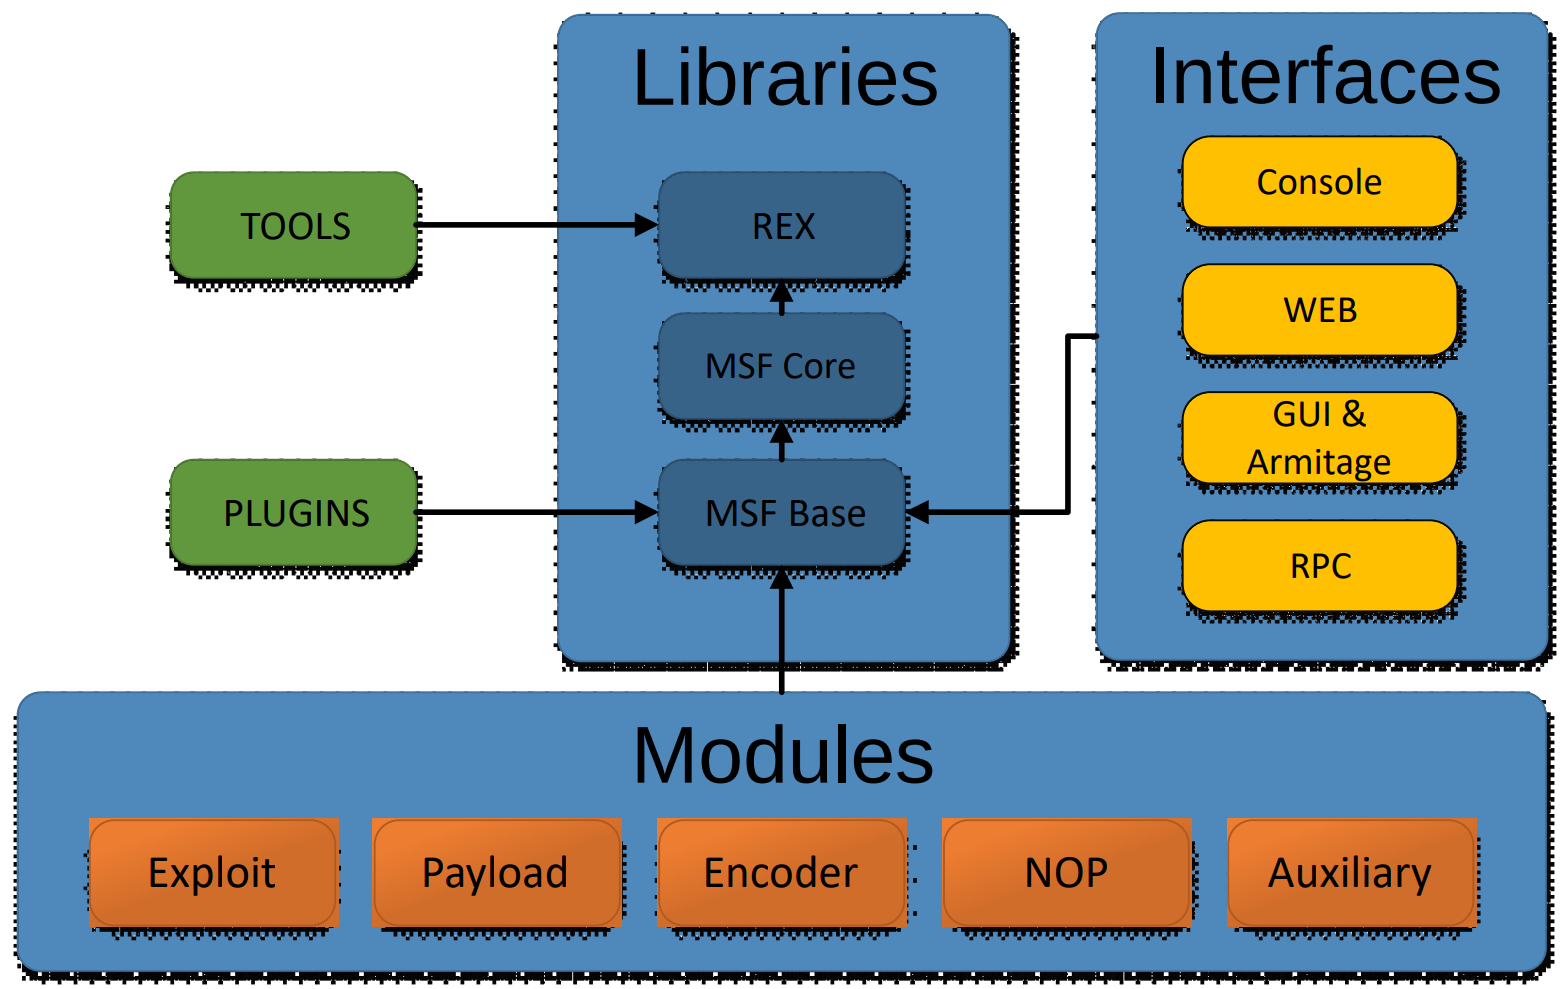
\includegraphics[scale=0.3]{images/SchemaMetasploit.png}
    \caption{Schema funzionale}\label{fig:1}
\end{figure}
\paragraph{Definizione exploit:} \\
Un exploit è una tipologia di script, virus, worm, porzione di dati o binario che sfrutta un bug 
o una vulnerabilità per creare comportamenti non previsti in software, hardware, o in sistemi elettronici, 
ad es. per ottenere l'accesso a sistemi informatici, permettere l'acquisizione dei privilegi amministrativi, 
o attacchi denial of service (DoS o il correlato DDoS). \\\\
\textbf{I passaggi fondamentali per l'exploiting di un sistema utilizzando Metasploit Framework comprendono:}
\begin{enumerate}
    \item Scegliere e configurare un \textbf{exploit} (codice che penetra in un sistema sfruttandone i bugs). 
    \item Controllare se il sistema attaccato è suscettibile all’exploit selezionato (facoltativo).
    \item Scegliere e configurare un \textbf{payload} (codice da eseguire sul sistema attaccato dopo esserci 
    penetrati con successo; per esempio una shell remota o un VNC server).
    \item Scegliere la tecnica di codifica in modo che l’intrusion prevention system (IPS) ignori il payload 
    codificato. 
    \item Eseguire l’exploit.
\end{enumerate}
\subsubsection{Metasploit Auxiliary Modules}
\begin{itemize}
    \item Exploit senza payload
    \item Scanning: tecnica per ricercare e mappare le debolezze di un'applicazione, di un computer o 
    di una rete
    \item Fuzzing: è una tecnica usata per individuare errori o falle di sicurezza del software. Il tester
     (o fuzz) invia al sistema dati casuali allo scopo di causarne il crash.
     \item Fingerprinting: generazione di una sequenza alfanumerica o stringa di bit di lunghezza prefissata 
     che identifica un certo file con le caratteristiche intrinseche stesse del file.
     \item Automated task
\end{itemize}



\subsection{Pratica}

\section{Fibra ottica}

\section{Buffer overflow}
\subsection{Teoria}

\subsection{Pratica}

\section{Reverse Code Engineering}

\subsection{Teoria}

\subsection{Pratica}

\subsubsection{Reverse APK}

\subsubsection{Reverse EXE}

\section{Honeypot e Honeynet}
\subsection{Teoria}

\subsection{Pratica}

\section{Darknet, Traffic Analysis and Botnet Trends}

\section{Challenge}


\section{Casi interessanti}

\subsection{Hacking Team}

\subsection{Carbanak}

\subsection{Oceanlotus}

\subsection{Wannacry}

\end{document}
